% Intended LaTeX compiler: pdflatex
\documentclass[preprint,12pt]{elsarticle}
\usepackage{graphicx}
\journal{Computer Physics Communications}
\usepackage[utf8]{inputenc}
\usepackage[T1]{fontenc}
\usepackage{lmodern}
\usepackage{microtype}
\makeatletter
% The class footer box is followed by a space token.
% The output routine then packs that box to \textwidth, and the space makes the line 2.6pt overfull.
\def\ps@pprintTitle{%
     \let\@oddhead\@empty
     \let\@evenhead\@empty
     \def\@oddfoot{%
       \hbox to \textwidth{%
        \ifnopreprintline\relax\else
        \@myfooterfont
         \ifx\@elsarticlemyfooteralign\@elsarticlemyfooteraligncenter
           \hfil\@elsarticlemyfooter\hfil
         \else
         \ifx\@elsarticlemyfooteralign\@elsarticlemyfooteralignleft
           \@elsarticlemyfooter\hfill{}%
         \else
         \ifx\@elsarticlemyfooteralign\@elsarticlemyfooteralignright
           {}\hfill\@elsarticlemyfooter
         \else
               Preprint submitted to \ifx\@journal\@empty
                 Elsevier%
            \else\@journal\fi\hfill\@date\fi
         \fi
         \fi
         \fi
       }%
     }%
     \let\@evenfoot\@oddfoot}
\makeatother
\usepackage{amssymb,amsmath}
\usepackage{xurl}
\usepackage{hyperref}
\usepackage{xr-hyper}
\externaldocument{rg_main}
% elsarticle 3.3 expands affiliation fields and breaks the accent in authors.tex.
\ExplSyntaxOn
\DeclareDocumentCommand \ca_aff_city { O{,} m }
  {
    \csgappto { ca_affiliation_values } { \unexpanded{#2} #1\ca_affitem_postskip }
  }
\ExplSyntaxOff

\date{\today}
\title{Supplementary material for CON 3.1}
\hypersetup{
 pdfauthor={Rohit Goswami},
 pdftitle={Supplementary material for CON 3.1},
 pdfkeywords={checkpoint, specification, restart, saddle},
 pdflang={English}}
\begin{document}

\begin{frontmatter}
%% elsarticle author block. One affiliation.
\author[tt]{Rohit Goswami\fnref{orcid}}
\ead{rgoswami@ieee.org}
\fntext[orcid]{ORCID: 0000-0002-2393-8056.}
\affiliation[tt]{organization={TurtleTech ehf.},
            city={Reykjav\'ik},
            country={Iceland}}

\begin{abstract}
These notes record the measurements behind the figures that accompany the CON 3.1 paper.
Each section is the one named from the main text.
The numbers are reads of the campaign files, the conformance corpus and the stored thread sweep.
\end{abstract}
\end{frontmatter}

\section{Restart difference}
\label{sec:supp-restart}
The interrupted band in Section~\ref{sec:validation} writes a checkpoint and then continues.
Figure~\ref{fig:supp-restart} compares each resumed movie with the uninterrupted movie at the same index.
Column 3 is that checkpoint.
The final column is the band after the five steepest-descent steps.

\begin{figure}[ht]
\centering
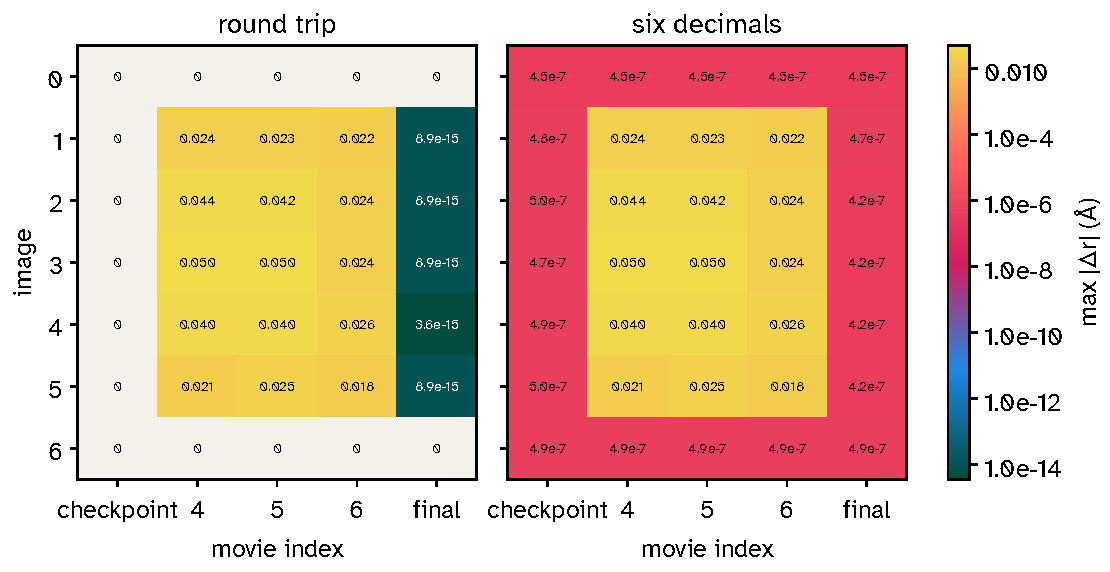
\includegraphics[width=\textwidth]{figures/generated/restart_diff.pdf}
\caption{Minimum-image maximum component of the displacement, in \AA, between the uninterrupted Morse band and each resume.
The checkpoint column is bitwise exact for the round-trip printer and about \(5\times10^{-7}\,\text{\AA}\) for six decimals.
The final column is at most \(8.9\times10^{-15}\,\text{\AA}\) for the round trip and \(4.9\times10^{-7}\,\text{\AA}\) for six decimals.
Intermediate columns differ by up to \(0.050\,\text{\AA}\) because the search has taken further steps after the load.
The colour scale is shared, and a zero cell is exact.}
\label{fig:supp-restart}
\end{figure}

\section{Round-trip fidelity}
\label{sec:supp-fidelity}
The comparison writes the velocity fixture through readcon and through ASE 3.29.0, then reads it back.
The adatom mask on the measured copy is 1, an x-only flag.
The stored velocity fixture itself uses mask 0 on that atom.
An id counts as kept only when the file that comes back still carries an id array.

\begin{figure}[ht]
\centering
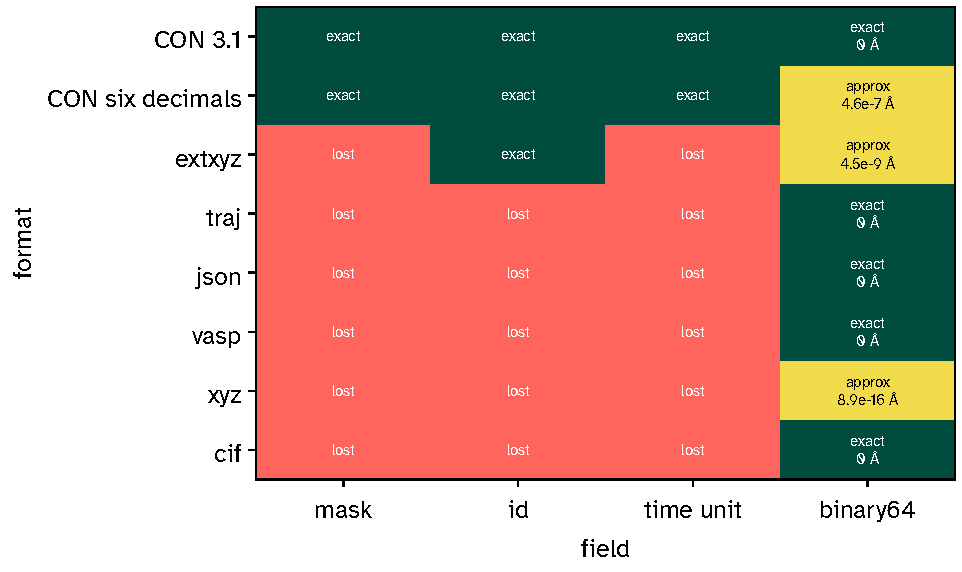
\includegraphics[width=0.92\textwidth]{figures/generated/roundtrip_fidelity.pdf}
\caption{Fields kept by a write and a read of the 28-atom velocity fixture.
CON 3.1 is the only format that keeps the mask, the id, the time unit and binary64 together.
The six-decimal CON writer keeps the mask, the id and the time unit, and moves a coordinate by at most \(4.6\times10^{-7}\,\text{\AA}\).
Extended XYZ keeps the id.
Every ASE format loses the per-axis mask.
The number in the binary64 cell is the maximum absolute coordinate change.}
\label{fig:supp-fidelity}
\end{figure}

\section{Frame bytes and parse time}
\label{sec:supp-anatomy}
The frame is the 28-atom velocity file, 3{,}826 bytes.
The timed files are 400 copies of that frame and 400 copies with the velocity section removed.
The reported times are medians of 31 paired reads.

\begin{figure}[ht]
\centering
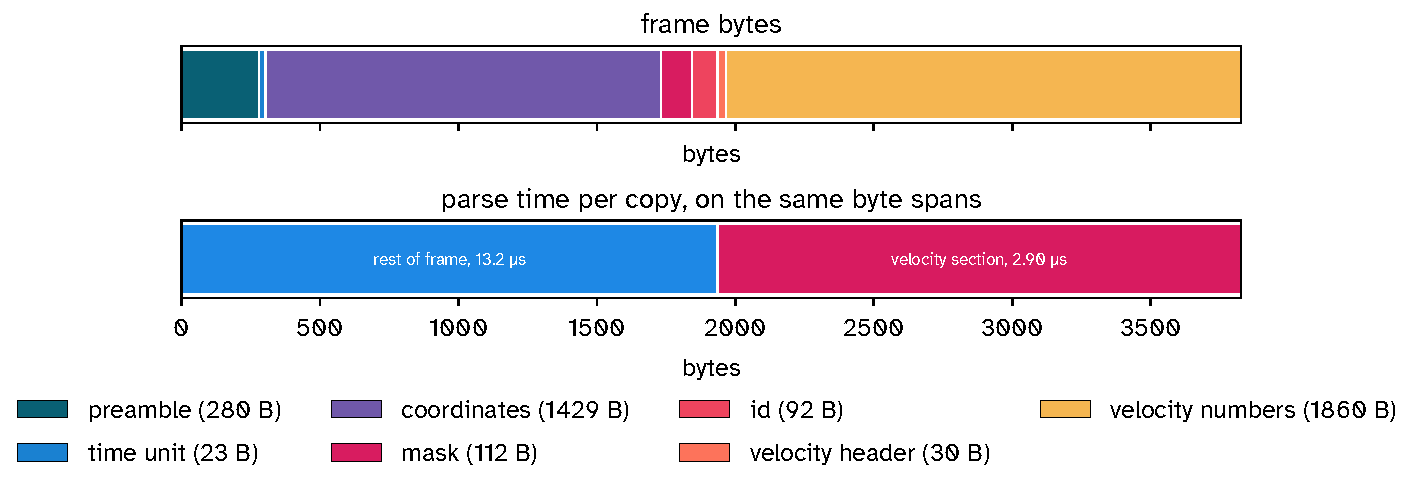
\includegraphics[width=\textwidth]{figures/generated/frame_anatomy.pdf}
\caption{Byte widths of one CON 3.1 frame, and the parse time of the same spans.
Masks, ids and the time unit are 227 bytes, against 1{,}429 coordinate bytes and 1{,}860 velocity-number bytes.
The velocity section adds \(2.90\,\mu\mathrm{s}\) to a \(13.2\,\mu\mathrm{s}\) read of the rest of the frame.
Masks and ids share the coordinate line, so their parse time is inside that \(13.2\,\mu\mathrm{s}\).}
\label{fig:supp-anatomy}
\end{figure}

\section{Velocity mislabel}
\label{sec:supp-velocity}
The kinetic energies and the Verlet step are the illustration in Section~\ref{sec:validation}.
The conversion from the natural unit to femtoseconds is the factor used for that illustration.
The cell is the slab cell of the file.

\begin{figure}[ht]
\centering
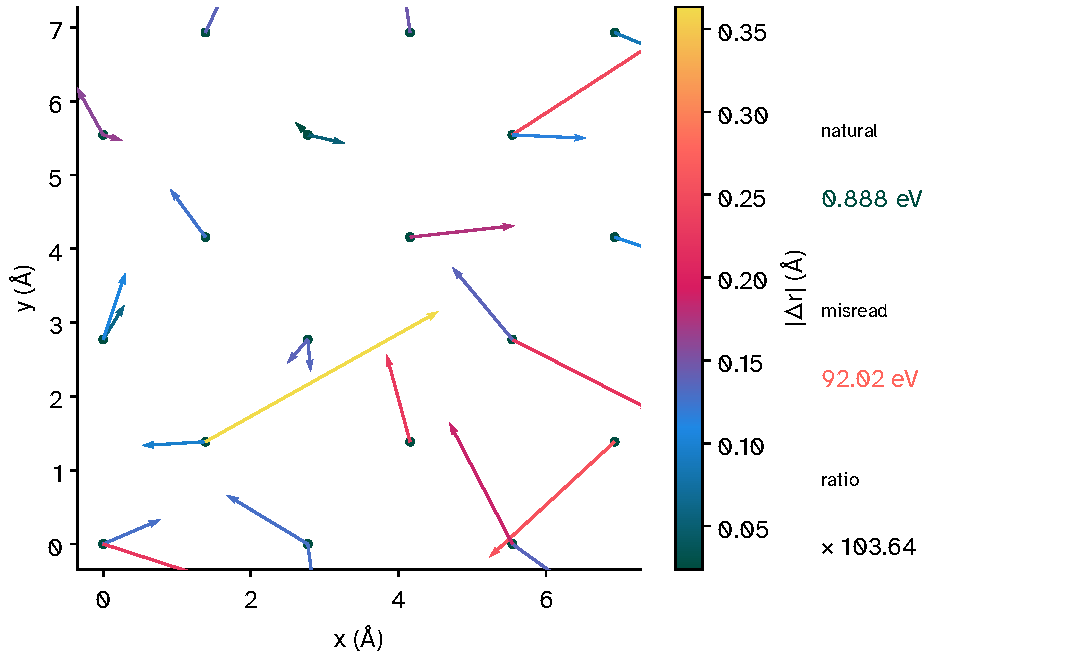
\includegraphics[width=\textwidth]{figures/generated/velocity_mislabel.pdf}
\caption{Displacement after one velocity Verlet step of \(1\,\mathrm{fs}\) on the 28-atom slab when the natural velocity is misread as \(\text{\AA}/\mathrm{fs}\).
The kinetic energy goes from \(0.888\,\mathrm{eV}\) to \(92.02\,\mathrm{eV}\), a factor of 103.64.
The RMSD is \(0.096\,\text{\AA}\) and the maximum component is \(0.315\,\text{\AA}\).
The arrows are drawn at 10 times that displacement, and the colour is the length of the displacement.}
\label{fig:supp-velocity}
\end{figure}

\section{Illegal-file classes}
\label{sec:supp-errors}
The eight illegal files are the conformance corpus named in Section~\ref{sec:validation}.
readcon raises a message that names the class.
The C bulk read, the iterator in Section~\ref{sec:implementation}, returns a null handle.
ASE 3.29.0 reads the same files with its eon reader.

\begin{figure}[ht]
\centering
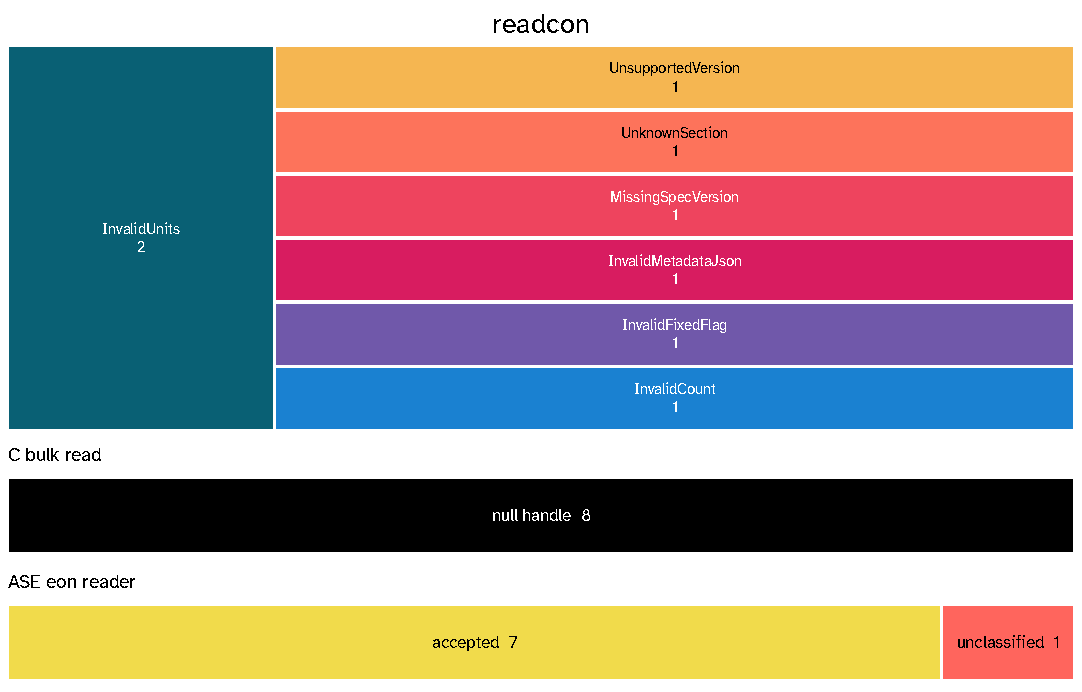
\includegraphics[width=\textwidth]{figures/generated/error_classes.pdf}
\caption{Classes on the eight illegal files.
readcon names a class for each file.
The C bulk read returns a null handle on all eight.
The ASE eon reader accepts seven of the files and raises an unclassified error on the per-type count of zero.}
\label{fig:supp-errors}
\end{figure}

\section{Distributed frame ownership}
\label{sec:supp-mpi}
A distributed read would assign each rank a contiguous block of frames.
The present code defines that partition.
It does not record the byte offset of each frame or the time spent on each rank.
This section has no figure.

\section{Hashed band geometries}
\label{sec:supp-dedup}
The hashes below are computed from the campaign geometries in this paper.
Each hash covers the coordinate array and the mask.
The five bands are the uninterrupted Morse restart, its round-trip resume, its six-decimal resume, and the two EMT mask bands of Section~\ref{sec:validation}.

\begin{figure}[ht]
\centering
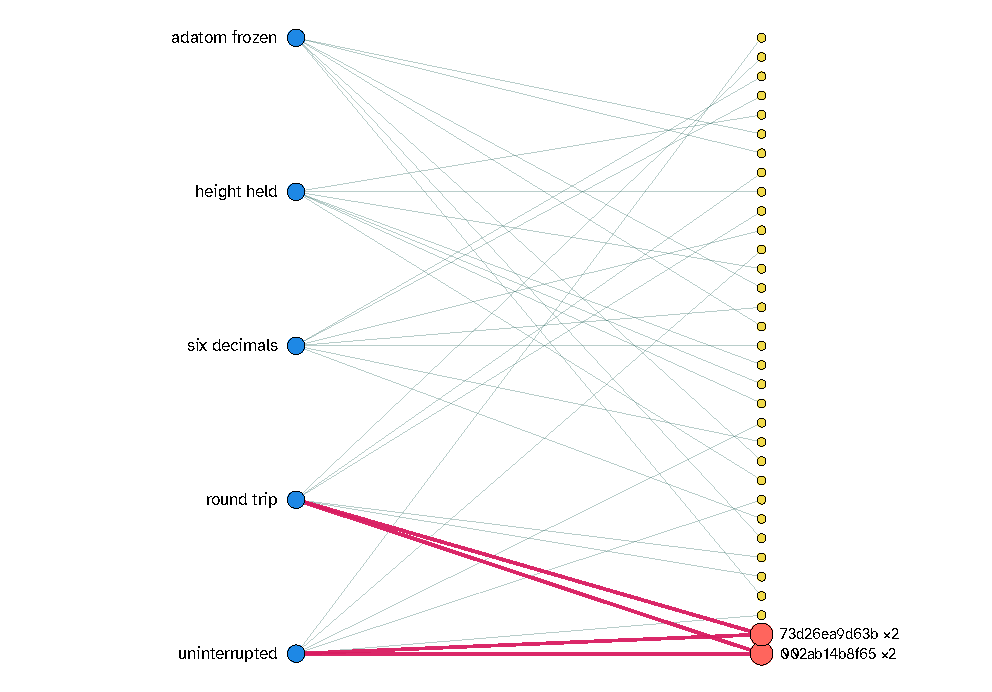
\includegraphics[width=0.86\textwidth]{figures/generated/dedup_graph.pdf}
\caption{Runs on the left and coordinate-and-mask hashes on the right.
The 35 images collapse to 33 hashes.
The two shared hashes are the endpoints common to the uninterrupted Morse band and the round-trip resume, and each of those hashes occurs twice.}
\label{fig:supp-dedup}
\end{figure}

\begin{figure}[ht]
\centering
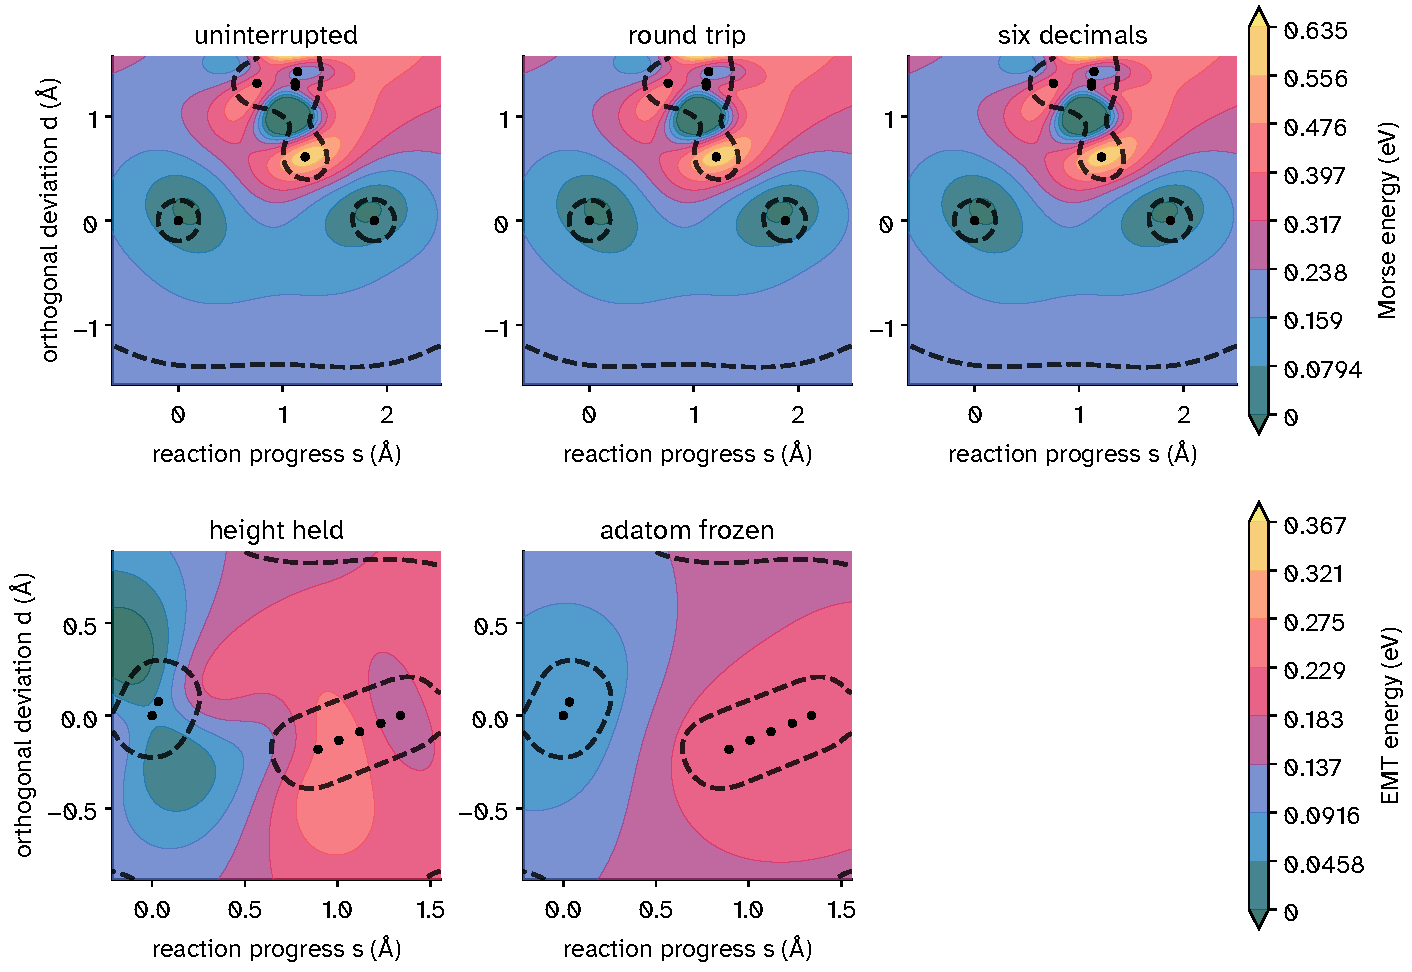
\includegraphics[width=\textwidth]{figures/generated/neb_multiples.pdf}
\caption{The same five bands on the \((s, d)\) plane \cite{goswamiTwodimensionalRmsdProjections2026}.
The Morse maps share one colour scale and the EMT maps share another.
Black dots are the images.
The round-trip and six-decimal maps sit on the uninterrupted Morse band at this scale, which is the agreement in Section~\ref{sec:supp-restart}.}
\label{fig:supp-neb}
\end{figure}

\bibliographystyle{elsarticle-num}
\bibliography{rg_main}

\end{document}
